\documentclass{thesis}

% clickable, breakable links
\usepackage{hyperref}
\usepackage{breakurl}

% better itemize
\usepackage{enumitem}
\usepackage{listings}
\usepackage{xcolor}

% Better captions
% TODO make sure caption size isn't TOO small
\usepackage[font=footnotesize,labelfont=bf]{caption}

% show author information in pdf document properties
\hypersetup{
	pdftitle={Tinzenite},
	pdfauthor={\thefullname}
}

% not sure for what this is here...
\colorlet{punct}{red!60!black}
\definecolor{background}{HTML}{EEEEEE}
\definecolor{delim}{RGB}{20,105,176}
\colorlet{numb}{magenta!60!black}

%JSON listing syntax highlighting support
\lstdefinelanguage{json}{
	basicstyle=\ttfamily\scriptsize,
	numbers=left,
	numberstyle=\scriptsize,
	stepnumber=1,
	numbersep=8pt,
	showstringspaces=false,
	breaklines=true,
	frame=lines,
	backgroundcolor=\color{background},
	tabsize=2,
	literate=
	*{0}{{{\color{numb}0}}}{1}
	{1}{{{\color{numb}1}}}{1}
	{2}{{{\color{numb}2}}}{1}
	{3}{{{\color{numb}3}}}{1}
	{4}{{{\color{numb}4}}}{1}
	{5}{{{\color{numb}5}}}{1}
	{6}{{{\color{numb}6}}}{1}
	{7}{{{\color{numb}7}}}{1}
	{8}{{{\color{numb}8}}}{1}
	{9}{{{\color{numb}9}}}{1}
	{:}{{{\color{punct}{:}}}}{1}
	{,}{{{\color{punct}{,}}}}{1}
	{\{}{{{\color{delim}{\{}}}}{1}
	{\}}{{{\color{delim}{\}}}}}{1}
	{[}{{{\color{delim}{[}}}}{1}
	{]}{{{\color{delim}{]}}}}{1},
}

% define special arrow list for model
\newlist{modellist}{itemize}{4}
\setlist[modellist]{label=$\multimap$}

% title definition
\fullname{Tamino P.S.M. Hartmann}
\email{tamino.hartmann@uni-ulm.de}
\headline{Tinzenite\\{\Large Encrypted Peer to Peer File Synchronization\\via the Tox Protocol}}
\titel{Thema}
\jahr{2015}
\matnr{722891}
\gutachterA{Professor Doctor Manfred Reichert}
\gutachterB{Professor Doctor Martin Theobald}
\betreuer{Marc Schickler}
\typ{Master thesis}
\fakultaet{Engineering, Computer Science, and Psychology}
\institut{Institute of Databases and Information Systems}

\license{
This work is licensed under the Creative Commons.
Attribution-NonCommercial-ShareAlike 3.0 License. To view a copy of this
license, visit \url{http://creativecommons.org/licenses/by-nc-sa/3.0/de/} or send a
letter to Creative Commons, 543 Howard Street, 5th Floor, San Francisco,
California, 94105, USA. \\ Setting: PDF-\LaTeXe
}

% hyphenations:
\hyphenation{Ta-mi-no}
\hyphenation{Hart-mann}

% DOCUMENT
\begin{document}

\frontmatter
\maketitle
\clearpage
\impressum

\cleardoublepage
\setstretch{1.2}	% original value: 1.4

\section*{Abstract}
\label{chap:abstract}

We proposed and implemented an open source, peer to peer, file synchronization tool based on the Tox protocol.
Targeted features include full secure communication between peers, optional encrypted peers, a server peer for third party support, and a focus on ease of use.
The software suite was implemented based on the Tox protocol, with Golang as the programming language, and the server client built on top of Hadoop.

TODO: Correct, improve, add.

\cleardoublepage
\section*{Gratitude}
\label{chap:gratitude}

My gratitude goes out to my support network from my university, my family, and my friends.
Especially my supervisor Marc Schickler for offering encouragement and praise when things worked -- I appreciate the support.
He also offered up excellent points for improving my thesis in his corrections.
My extended family for the many nice questions about what I was doing and sitting through the long explanations with sufficient interest to keep me going.
Maybe someday I will find a single sentence that sufficiently explains everything comprehensibly for "non-computer" people.
My aunt Sibille and my parents Katja and Stefan for their hard work of proof reading this thesis: all remaining errors are my own.
Furthermore my friends for regularly asking how I was doing, thus building up the pressure to keep working continuously.

This work would not have been possible without the great tools and libraries and the many people that implemented and documented them.
Therefore my heartfelt thanks go out first and foremost to the open source community that made building this thesis a possibility: Tox for providing a peer to peer fully encrypted communication channel and Golang for the access to source code when things didn't work as expected.
Worthy of special mention is the Github user Codedust for maintaining the Golang Tox wrapper on which I built this thesis.
Special thanks are due for their support whenever I had problems or feature requests and always received help and support.


%TODO set good depth level. 3 seems to be too much but required for ease of access while I'm still writing the document.
\tableofcontents

\mainmatter

\chapter{Introduction}

Test text to test some testing text.
Notably, she said: "Doubtly so, Mr. Bond, but can you live?"
Laughing out loud, test done~\cite{web:site:tox}.

\chapter{Related and Existing Work}
\label{chap:Related and Existing Work}

This chapter serves two purposes.
First we will discuss existing solutions.
The differences between these and our proposed work will serve to highlight in what ways our work expands existing solutions.
Then we will take a look at the academic side of file synchronization and discuss related papers.
These will serve as a foundation for how we implement the Tinzenite protocol.

\section{Existing Software}
\label{sec:Existing Software}

\begin{figure}[htp]
\centering
    \includegraphics[width=0.3\linewidth]{diagram/topo_s2c}
    \hspace{2em}
    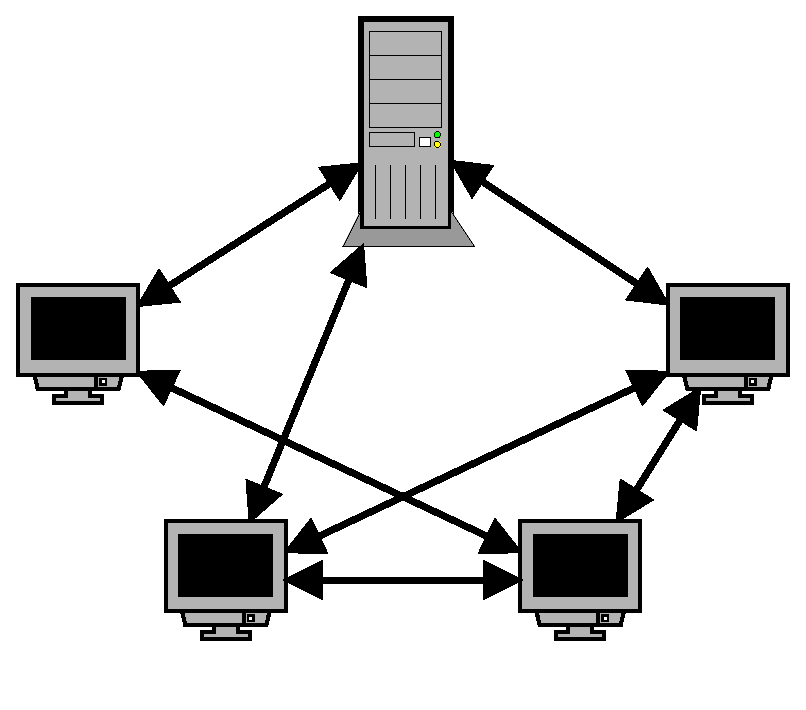
\includegraphics[width=0.3\linewidth]{diagram/topo_p2p}
\caption[Example Network Structures]{Example diagrams of a server client architecture (left) and a peer to peer architecture (right). Note that the peer to peer architecture does not exclude servers as peers.}
\label{fig:example_netarch}
\end{figure}

For any internet technology there are two options for how to structure its architecture in general.
Most of the internet today is cleanly divided in a client-server structure where a client always requests information from a central server.
This is a strongly hierarchical structure.
An example of this is downloading a PDF from a website.
The other option is a distributed peer to peer model, where a client requests information from any other client and in turn will also respond to queries from other clients.
One of the more well known candidates of this is the Bittorrent protocol~\cite{web:site:bittorrent}.
Both options have been used in existing file synchronization solutions.
See figure~\ref{fig:example_netarch} for an example diagram of the two architectures.
Therefore we have divided the existing software we will shortly discuss in the following sections between these two extremes.

\subsection{Client-Server Solutions}
\label{sub:Client-Server Solutions}

For client-server solutions any user must rely on the availability of the central server.
These are often hosted by third parties in a distributed manner for reasons of performance and scaling.
Providing a central service that is required for the file synchronization to work also allows easy monetization.
Since a large amount of such services exist, we will highlight only the three most popular ones for this thesis.
These are respectively: Dropbox with 300 million users, Microsoft's OneDrive with 250 million users, and Google Drive with 240 million users as of 2014~\cite{web:site:fortune}.

\subsubsection{Dropbox}
\label{subs:Dropbox}

Dropbox~\cite{web:site:dropbox} is one of the most popular cloud storage providers currently and is known by many users looking for a solution that works across multiple operating systems.
Positive features include web access to stored data, clients for many different platforms, easy sharing of data with outsiders, and ease of use.
On the negative side the service relies on its back-end servers, although computers can synchronize files between themselves on a local area network.
Dropbox also lacks any end to end encryption, but does encrypt data while in transit and when "at rest" in their data centers~\cite{web:site:dropbox:blog}.
Therefore it comes with little surprise that they were prominently featured in the Snowden leaks~\cite{web:site:rt:dropbox}.
The company does have full access to any data the user uploads to their servers, as long as the users do not encrypt the files beforehand themselves.
Therefore we can extrapolate that Dropbox can offer up a user's data if required to by a fourth party, as is the case in the United States of America.

Dropbox offers a free account for a basic storage plan.
Additional storage capacity is available for purchase.
None of the core applications have been open sourced to date, meaning even if Dropbox implemented strong encryption it could not be independently verified.

\subsubsection{OneDrive}
\label{subs:OneDrive}

With the release of Microsoft's newest operating system the company has increased its push for public adoption of its OneDrive~\cite{web:site:onedrive} cloud storage service.
It is now directly integrated within Windows 10 and is opt-out for users that do not wish to utilize it.
OneDrive is integrated with Microsoft's answer to Google Docs, Office 365.
Furthermore more free storage is added for registering devices and using Microsoft's products.

Similar to its two competitors, the base plan is free, with the option of paying monthly for an increase in storage space.
No software for OneDrive has been open sourced.

\subsubsection{Google Drive}
\label{subs:Google Drive}

Google Drive~\cite{web:site:gdrive} is similar to Dropbox in term of its functionality.
It does go a step further than Dropbox by integrating tightly with their suite of online applications for creating and editing documents, named Google Docs.
Google also has full access to all data that users upload to their servers.
This in turn means that under the PRISM program by the NSA, all such data is also retrievable by a fourth party~\cite{web:site:rt:google}.

Google also offers a basic storage amount at no charge for the user.
Again additional space can be purchased on a monthly basis.
Apart from offering access to fewer clients than Dropbox, Google also has failed to open source the components of its service.

\subsection{Peer to Peer Solutions}
\label{sub:Peer to Peer Solutions}

Peer to peer systems work without a central server.
The trade off is that such solutions require assistance in locating other peers, which means that some form of a peer discovery system must be implemented.
While this could be done via a central server, nowadays the common solution to the problem is a distributed hash table~\cite{ratnasamy2001scalable} which is used to look up the required peers.
Once another peer has been found the connection can be established.
Apart from not relying on the availability and trustworthiness of a central server, peer to peer solutions offer a possible performance advantage as they can distribute bandwidth between every peer, even actively unchoke a saturated peer.
As an added bonus the path data takes between two peers will always be the most direct path as no data must first go towards a third party.
This bonus can be lost if onion routing is implemented for anonymity purposes.

\subsubsection{BitTorrent Sync}
\label{subs:BitTorrent Sync}

An existing solution for a peer to peer data synchronization service is Sync~\cite{web:site:bittorrent_sync} from the BitTorrent company.
It is built on existing BitTorrent technology and thus keeps many of the positive features associated with BitTorrents: reducing the impact of transferring large files over a limited network.
Therefore it has no central point of failure and can even run without internet access by transferring files between computers on a local area network directly.
However, just as the client-server solutions before, Sync is closed source.

Clients exist for a multitude of platforms.
While information is encrypted in transfer, there is no differentiation for untrusted clients.
Sync is free for basic usage, but requires a paid account for additional features that offer more fine grained control.

\subsubsection{Syncthing}
\label{subs:Syncthing}

Syncthing~\cite{web:site:synthing} is an open source file synchronization software on an equally free block exchange protocol.
This protocol is a mixed data transfer and communication protocol in one, with encryption for all communication built in directly.
Again the user can not designate untrusted peers.

Unlike the other solutions mentioned here, Syncthing is open source and can thus be independently verified to be secure.
Like Tinzenite it is also implemented in Golang.
The downside is that Syncthing lacks a feature which BitTorrent Sync shares with most client-server solutions: the capability of sharing a specified file or directory with other users who are not part of the storage system.

\subsection{Additional Security Layers}
\label{sub:Additional Security Layers}

It is of course possible to encrypt all data before using any data storage service beforehand.
This has a few notable downsides however.
For many client-server solutions the user loses out on web access to the data along with a host of additional feature built on the availability of the data.
While advanced users may be capable of encrypting their data themselves using a range of available tools, such solutions require the user to manage the encryption keys themselves.
This is a non trivial issue beyond adding an additional hurdle to using data storage services.
As so often commercial solutions for this exist.

\subsubsection{Boxcryptor}
\label{subs:Boxcryptor}

All three server-client services mentioned are not to be trusted with private information that must remain secure due to possible fourth party access.
However solutions for encrypting the data sent over such services which manage the encryption keys exist.
One example of such a service is the Boxcryptor software~\cite{web:site:boxcryptor}.
It encrypts all data before uploading it to the connected cloud storage service and decrypts it when retrieving it.
The user keys are attached to the user's account.
Asymmetric encryption is used to upload all keys to the companies key server so that other clients can retrieve and, with a correct password, decrypt the data.
Sharing of data is still possible even for users without an account by utilizing special keys.

The downside to this approach is mainly that it has to be used on top of an existing cloud storage service.
This effectively means that the user must run an additional program on top of the file storage service to ensure secure data.
Boxcryptor can be used with most existing third party data storage systems.
Boxcryptor offers a free version of its service, but to access all security features a paid subscription is required.
The software is not open source and thus not independently verifiable.

\subsection{Comparison}
\label{sub:Comparison}

In this section we will briefly highlight the capabilities and differences between the discussed existing solutions.
We chose to compare the features that we believe to be most important to this thesis.
See table~\ref{table:software_comparison}.

\begin{table}[htp]
\begin{threeparttable}
\centering
{\small
\begin{tabulary}{\textwidth}{ L || c | C | C | C | C }
    \textbf{Name} & \textbf{Architecture} & \textbf{Free Storage} & \textbf{Client-side Encryption} & \textbf{Open Source} & \textbf{Account Required} \\
    \hline \hline
    Dropbox & Centralized & 2 GB & & & \checkmark \\
    \hline
    OneDrive & Centralized & 15 GB & & & \checkmark \\
    \hline
    Google Drive & Centralized & 15 GB & & & \checkmark \\
    \hline
    Boxcryptor & --\tnote{a} & --\tnote{b} & \checkmark & & \checkmark \\
    \hline
    BitTorrent Sync & Distributed & $\infty$ & & & \checkmark \\
    \hline
    Syncthing & Distributed & $\infty$ & & \checkmark & \\
\end{tabulary}
}
\scriptsize{
\begin{tablenotes}
    \item[a] Boxcryptor is used on top of an existing cloud storage provider.
        The encryption infrastructure itself is centralized.
    \item[b] Boxcryptor is free to use but many features are only available for a paid account.
\end{tablenotes}
}
\end{threeparttable}
\caption[Existing Software Comparison]{This table serves to highlight the differences between the existing software previously discussed.}
\label{table:software_comparison}
\end{table}

\section{Related Research}
\label{sec:Related Research}

The following discussion concerns papers that we believe have an impact on our work.
We discuss their general content with a focus on what information we extracted and how we believe we can apply it to Tinzenite.

\subsection{What is a File Synchronizer?}
\label{sub:What is a File Synchronizer?}

The paper by Balasubramaniam and Pierce~\cite{balasubramaniam1998file} has the stated goal of offering a framework for describing the behavior of file synchronizers.
Notably the paper's authors divide the process into two separate phases: update detection and reconciliation.
Update detection is defined as the recognition of where updates have been made to the directory since the last synchronization.
Reconciliation is defined as the combination of updates between peers to transfer all peers to a new, synchronized state.

For Tinzenite we assimilated a few things out of this paper: primarily the distinction between the update detection and the reconciliation phase.
We will also initially ignore links and file permissions due to increased complexity, but unlike them we will never modify a file ourself.
The paper also gave us a definition for the type of update detection strategy we wanted to try: namely the modtime inode strategy.
Ideally we would take an on-line update detector but this seems impossible to do under Linux currently for an unlimited amount of files.
Also of interest is the differentiation between pull and push models for propagating updates.
Tinzenite intends to be a hybrid between the two: while the main work will be done via push -- once peers have established a connection -- updates may also be propagated via pull for performance reasons.
In the reconciliation section of the paper is the listing of the various possible states that two replicas of a directory can possibly reach given a set of operations, which is also of interest for this thesis.
We intend to ensure that the core protocol for Tinzenite will be capable of handling all of them to the best of its abilities.

\subsection{An Algebraic Approach to File Synchronization}
\label{sub:An Algebraic Approach to File Synchronization}

The paper by Ramsey and Csirmaz~\cite{ramsey2001algebraic} presents an algebra for reasoning about file system operations with the intended purpose of specifying an algorithm for file synchronization.
Interesting for our work is the discussion of possible commands that can be executed on said file algebra.
While from a user's point of view a multitude of operations seems possible (create, remove, rename, move, derive, and edit) the paper's authors distill these down to just three for the technical side: create, remove, and edit.
Rename can be executed by removing the original file and creating a new file with the new name while keeping the content identical.
Move can be executed much the same but keeps the name, instead changing the location where the new file is created.
Derive is argued to be indistinguishable from edit without higher level knowledge.
While not impossible to detect, this feature we consider to be beyond the scope of Tinzenite.
Features that Tinzenite shares with the paper's prototype include that parents must be created before their children and that children must be removed before their parents.

The paper also offers a number of improvements that Tinzenite could incorporate.
Notably this includes support for an explicit move command.
This would remove the need for removing and recreating a file's content when it was moved, thus making this operation more performant.% performant is written correctly
They also suggest using fingerprints of content to avoid sending data that already exists.
Tinzenite already utilizes content hashes, so expanding it to be more intelligent about when to request actual data to be sent should be easily implementable by comparing hashes of files before requesting transfers.

\subsection{Peer-to-Peer Reconciliation Based Replication for Mobile Computers}
\label{sub:Peer-to-Peer Reconciliation Based Replication for Mobile Computers}

In~\cite{reiher1996peer}, Reiher et al. nicely state the benefits and drawbacks of using a peer to peer system for file synchronization in regard to mobile devices.
Benefits include not having to rely on an permanently available server, being able to transfer files without access to a central server, and transferring files over the shortest available network path.
The authors list as drawbacks the higher required complexity of the algorithms used to control the replication.
They conclude that peer to peer replication is well suited for mobile devices.

\subsection{Perspectives on Optimistically Replicated, Peer-to-Peer Filing}
\label{sub:Perspectives on Optimistically Replicated, Peer-to-Peer Filing}

The paper by Page et al.~\cite{page1998perspectives} is notable in our case for two main reasons.
It offers a nice set of definitions of problems that we must also solve for Tinzenite and even offers relevant solutions.
The authors also discuss the performance of their implementation.
Focus of the paper is the evaluation of the use of optimistic replica consistency, automatic update conflict detection and repair, the peer to peer interaction model, and the Ficus design and construction.

Relevant for Tinzenite is the paper's solution to the insert delete ambiguity.
The solution is to keep a list of deletions until all peers know of the deletion.
Only then can the deletion actually be garbage collected.
In Tinzenite we will use a similar approach.

\section{Conclusion}
\label{sec:Conclusion}

Based on the listed existing solutions and the briefly discussed related papers we have synthesized a set of features that we wish Tinzenite to have.
These will be discussed in the next chapter.
More importantly our research highlights a few problems that we will need to solve or use already existing solutions for.
This starts with defining the operations we will allow on objects within a directory and continue on to how to solve ambiguities and merge conflicts when synchronizing between multiple peers.

\chapter{Concept}
\label{chap:concept}

The following chapter discusses all conceptual work that went into creating Tinzenite.
We will first give an overview of the basic goals of this thesis.
Next we will expand on the goals by discussing the features we would like Tinzenite to have and defining their scope.
Then we will give an overview on the software we would like to build on.
Finally we will highlight the features and differences of each software aspect of the Tinzenite system.

\section{Basic Goals}
\label{sec:Basic Goals}

The stated goal of Tinzenite is to offer a peer to peer solution for file synchronization that builds on the strengths of Tox.
It is important to us to build the system in a way that it is secure from unauthorized access by third parties, even if they retain a copy of the data.
In fact we propose an explicit client for third party support so that third parties can offer a storage peer as a service.

Therefore we will need to develop a protocol for a decentralized and distributed system that relies on the underlying secure channel provided.
It seems clear that to minimize developer work we will implement a reference software library for the core protocol.
Expanding on this we hope to implement a peer client for normal computers and a third party client that securely stores the user's data off site.

\section{Features}
\label{sec:Features}

This section will define the features we would like Tinzenite to have, including features that for now go beyond the scope of the thesis.
Therefore we will classify the features by scope for reference afterwards.
The exact features we would like to have have been synthesized from the existing and related work (see section~\ref{chap:Related and Existing Work}).

\begin{description}[leftmargin=2em,style=nextline,noitemsep,nolistsep]
\item[Protocol]
    Design of an extensible protocol on which all communication between peers will be based.
    We will specify the protocol as JSON encoded messages that will be sent as text messages via the Tox protocol.
    The open specification will allow the development of compatible peers by others, important for the extensibility of the system.
\item[Peer to Peer Architecture]
    The complete software suite should run in a direct peer to peer mode to remove the requirement of third parties to facilitate data exchange and to remove the associated security risk.
    This includes the server client as it should be capable of exchanging data even with other server clients.
    As the underlying Tox provides direct peer to peer connections this should be a given from the beginning.
    We also hope that this feature will allow clients to synchronize independently of the internet: peers should be capable of utilizing local connections directly.
\item[Secure Transport]
    All communication between all clients should always be fully end to end encrypted.
    This feature is also provided by the underlying communications software.
\item[Third Party Client]
    A dedicated client for third party servers that holds only an encrypted copy of the data.
    Notable features are that a single instance should handle multiple users' accounts.
    Since large data amounts are to be expected, the server client will be capable of integrating the Hadoop distributed file system to directly support that.
    Support for commercialization of a service based on this client will be provided.
    This includes size and amount distinction based on a per user basis.
    Notably this feature requires peers to authenticate themselves against each other if they are trusted peers.
\item[Shadow Files]
    It should be possible to avoid having to fetch unwanted files for space constrained clients.
    Dubbed shadow objects, this feature could be important for mobile devices as they run on power and bandwidth constraints.
\item[Delta Updates]
    Since it is wasteful to transfer redundant data when only small parts of files are changed, we would like to add the capability to only send the delta difference between two files.
    Note that this is not required for the core functionality but a nice to have optimization.
\item[Object Atomicity]
    We believe that the proposed system should concentrate on one thing and do it well\footnote{Also known as the Unix philosophy.}.
    Therefore we will not touch the content of files, instead treating them as singular objects.
    This should help to guarantee that files are never modified by the system beyond the required operations for synchronization.
    In particular this forbids automatically merging changes in files.
    All conflicts must be resolved by the user: we do not intend to guess the correct resolution strategy for any file type.
\item[Client Agnostic]
    As stated we propose to implement the core protocol functionality in a central library that can be used by different clients independent of their concrete purpose and implementation.
    Therefore we will implement the library as platform agnostic as possible, relying on clients to implement the required file operations and system calls as required.
\item[Concurrency]
    Building on one of the original goals of Golang, we plan on implementing the core library of Tinzenite in an efficient strategy by fully utilizing the language's built in concurrency.
    This should allow Tinzenite to make full use of multi core systems and avoid locking the library up should a single process lock up.
\item[Usability]
    Last but not least in any way we hope to implement reference software in a way that any user can, after the initial setup, use Tinzenite without complex interactions.
    Once the peers for a directory are setup Tinzenite should run as non-intrusive as possible while retaining the user's confidence in the reliability of the system.
    An example for a usability feature might for example be a way to easily authenticate newly connected peers via QR codes or word based hashes instead of the full Tox ID.
\end{description}

There are also features that would be nice to have but are beyond the goal of this thesis.
These include for example the ability to share single files within a synchronized directory with outside users, as seen in Google Drive or Dropbox for example.
This feature is excluded because it requires a more complicated security and encryption model that we do not feel capable of implementing securely.
Security is hard to do correctly, therefore we will limit ourselves before jeopardizing the security of the whole system.

Another feature that would be sensible to have is data obfuscation for encrypted peers.
This would make it even more difficult for nefarious services to extract any information from a hosted encrypted peer.
This would however require a more advanced and distinguished transmission mode for encrypted peers.
Furthermore data deniability is most definitely beyond the capabilities of the proposed implementation (and since the core goal of Tinzenite is data availabilty, somewhat contrary).
If a user allows full access to the directory to an untrusted party there is little that we can do to mitigate the security breach.

Please note that many further features are not dependent on the capability of the Tinzenite system but on the implementation of peers.
An example for this is web access to an encrypted storage: this is a feature that explicitly can be implemented in a secure way\footnote{The key for decrypting the data can be unlocked by the user in the web browser by entering the correct pass phrase. Utilizing the shadow file capability the web application would act as a temporary trusted peer until the user is done with his data access.}.
However we make no guarantee that we will get around to implementing it.

\subsection{Scope}

In this brief section we will go through the exact scope that this work is to fulfill.
We therefore divide the above features into three categories, ranging from required to have the thesis considered successful to those that can be added as extras.
Furthermore we we expand on the actual implementation work we intend for each scope definition.

\subsubsection{MUST Have}
\label{subs:MUST Have}

These features are required for the thesis to be considered basically successful.
This means that the basic fundamentals of the proposed complete scope have been met and are in working order.
Specifically this includes a fully working computer client based on a specified API on which all future work can be built on.
This client must offer the basics required to get the system to work in a user friendly manner from setup through daily usage.
Data transfer between multiple clients must work as expected with collision detection and correct version iteration upon updates.

\begin{description}[leftmargin=13em,style=nextline,noitemsep,nolistsep]
\item[Protocol]
    The core protocol must be fully capable of the basic file synchronization.
\item[Peer to Peer Architecture]
    The base client and library must be capable of running without a centralized system.
\item[Secure Transport]
    All communication must be fully encrypted.
\item[Object Atomicity]
    Files must not be modified by the system beyond the modifications required for the synchronization.
\end{description}

\subsubsection{SHOULD Have}
\label{subs:SHOULD Have}

Features in this category are features that built on the MUST have features and are thus not strictly required.
In broad terms this includes two important aspects.
First and foremost is the capability of having a client that only retains an encrypted version of the data.
Built on this the second aspect is the server client that only ever retains an encrypted data set.
The server also adds the capability of handling multiple users' data on a distributed file system capable of handling the large data size that are to be expected for multiple concurrent users.

\begin{description}[leftmargin=9em,style=nextline,noitemsep,nolistsep]
\item[Third Party Client]
    The capability of supporting encrypted clients should be implemented.
\item[Client Agnostic]
    This feature should be a given once we have started implementation of the second peer program.
\item[Usability]
    The base usage of Tinzenite should be trivial for most users from a usability perspective.
\end{description}

\subsubsection{COULD Have}
\label{subs:COULD Have}

These features are features that will only be implemented if all previous features have been successfully integrated.
They are not required for the thesis to be considered overly successful but would be nice to have to fully complete the proposed scope.
Primary aspects that would be added in this phase are a mobile client, most likely as an application for Android, and possibly even a web interface for accessing encrypted server clients.
A further smaller aspect would be shadow file capabilities so that data can be selectively synchronized on constrained devices, specifically mobile devices for example.

\begin{description}[leftmargin=7.5em,style=nextline,noitemsep,nolistsep]
\item[Shadow Files]
    Peers could be allowed to only fetch files that the user explicitly wishes to have synchronized on a peer basis.
\item[Delta Updates]
    Transfer times of files over limited bandwidths could be optimized by only transferring the differences between them.
\item[Concurrency]
    The core library could support communicating with multiple peers concurrently, thus working around bandwidth constraints.
\end{description}

\section{Dependencies}
\label{sec:Dependencies}

This section briefly highlights the technologies we chose to support our work.
These range from software solutions to data organization standards.

TODO: librsync for the delta file transfer?

TODO: Move this to related work, me thinks.
This has little to do with the concept directly but is a core pillar on what I'll be basing my work on.

\subsection{Tox}

TODO: list, explain

\subsection{Golang}

TODO: list, explain

\subsection{Hadoop}

TODO: list, explain

\subsection{JSON}

TODO: list, explain

\section{Software Scope}
\label{sec:Software Scope}

TODO: section for listing actual conceptual work I'll have to do before starting implementation.
Also consider implementing a working but "quiet" client – no file transfers but reads out communications.

TODO: Or, instead of a quiet client, just start with the protocol implementation before actually enabling Tinzenite to send files.

\subsection{Core Application Library}

TODO: all the core logic should be strictly kept separate from the user side of the software.
The library will encapsulate the JSON communication and states of said API.
Clients will have to register hocks for incoming updates, files, and notify the library of updated (delta) files.

To keep development of clients as easy as possible while at the same time keeping the API consisten between them we will separate the core logic for Tinzenite from any user oriented code.
Therefore the library will encapsulate the Toxcore library and build on it the core features required for clients to work.
This means that we will have to define a library API for interfacing with it.
The library will not handle writing or reading data from the user's disk: these capabilities will be offloaded to the implementation of the client programs.
This will ensure a maximum of adaptability for clients, meaning that they will not be constrained by the cross platform capabilities of the library itself.
%TODO of course, Toxcore might pose a problem here... :P

\begin{table}[H]
\centering
%TODO clean table formatting for use everywhere... :P
\begin{tabulary}{\textwidth}{p{2.5cm} || J}
	Initialize & Prepares Tinzenite and starts the underlying libraries, notably connects to the Tox network. Note that once initialized, files will be sent and written immediately. Settings and options must be handed over on initialization.\\
	\hline
    Register Callbacks & Given object will be called for all callbacks.\\
    %TODO: what callbacks should be specificed? register for all should be an option, but registering for any should be possible too!
\end{tabulary}
\caption[Tinzenite Library API]{Methods for accessing the Tinzenite library.}
\label{table:lib:api}
\end{table}

TODO: What about helper functions?
Should be cleanly separate too.
Notably probably includes delta of files, ...?, etc.

\subsection{Client Peer}

TODO: list and explain features of basic computer client (how to connect peers, how to encrypt), remember that usability is important.
Features: password protected everything as with TextSecure?
Visibility of operations is important.
Will also need to put some thought into support of shadow files – what exactly are they and what happens when I click on one?

\subsection{Server Peer}

TODO: write that basically encrypted peer that can handle multiple accounts, stores data via Hadoop.
Future work could include web client – should I add this here too?

\subsection{Mobile Peer}

TODO: write that App, add shadow file feature

\section{Security Considerations}
\label{sec:Security Considerations}

TODO: place all the security stuff here...
Also note how security has been implemented throughout the concept.
If I place it here I won't have to reexplain it in the architecture chapter.

The peer list is the more problematic of the two as it can be used to determine the size of the user's Tinzenite peer network.
However to allow encrypted peers to facilitate file transfer between two mutually exclusively online peers, it must know this information.
This is mitigated by the fact that Tox IDs are hard to guess and not shared beyond the Tinzenite peer network.

\chapter{Architecture}
\label{chap:architecture}

The following section will define the data model each peer keeps of its data and specify the API for updating it between peers, both trusted and encrypted.
Therefore we start this chapter with an explanation of all meta information that a trusted peer stores, as everything else is based on top of this information.
Then we will define and explain the model each peer keeps of the stored data.
Built on this model we will discuss the messages used to facilitate the update of the model between clients.
Then we will discuss the protocol extensions required for the encrypted model.
Finally we will take a look at the advanced features and how they can be built on top of the previous work.

We chose to use JSON for all communication between peers as further discussed in section~\ref{sub:JSON}.
Therefore generally speaking all messages will be defined as JSON messages.
Additionally most data is written to storage as JSON files.
This has the advantage of allowing easy manual access to all files and message for development purposes since JSON messages can be sent as simple text messages via the normal Tox chat clients.

\section{Meta Data}
\label{sec:Meta Data}

Since a trusted peer must store the last known state of the directory to detect changes for later synchronizations, we must store this information to storage somewhere.
For Tinzenite we took a page from Git and decided to write this information within the directory to be synchronized.
To reduce visual clutter and to hide it from users this directory is offered by a hidden directory directly below the root directory.
We specified it as \textit{".tinzenite"}.
In short it contains organizational files, temporary objects, and the deletion directory for storing files until they have been fully removed by all peers, plus data private to the peer.
Figure~\ref{list:meta_folder} gives a broad overview of the contents.

\begin{figure}[htp]
\begin{modellist}
\item .tinzenite/
\begin{modellist}
    \item org/
    \begin{modellist}
        \item peers/
        \item auth.json
    \end{modellist}
    \item removed/
    \item temp/
    \item receiving/
    \item sending/
    \item local/
    \begin{modellist}
        \item rmstore/
        \item model.json
        \item self.json
    \end{modellist}
    \item .tinignore
\end{modellist}
\end{modellist}
\caption[Meta Folder Structure]{Overview of the special meta information directory that Tinzenite uses to store relevant information required for the managing of the directory. For brevity sub directories that contain instance data are not expanded.}
\label{list:meta_folder}
\end{figure}

Placing the meta data within the directory has a few benefits for the complexity of the system and enables it to utilize the full feature set of the implemented synchronization capabilities to share data between peers when required.
Specifically only the \textit{"org"} directory and the \textit{"removed"} directory are synchronized as any user data, along with the \textit{".tinignore"} file which specifies to ignore all other objects.

\subsection{Organizational Directory}
\label{sub:Organizational Directory}

The \textit{"org"} directory consists of two objects: the file containing the authentication information and a sub folder which contains a file for each known peer.
It is first of two directories that are synchronized along with user specified files between peers, as both the authentication file and the peer list are required for all peers.

\subsubsection{Authentication File}
\label{subs:Authentication File}

The authentication file stores information required for the complete Tinzenite network.
This includes information on the user, the directory the network synchronizes, and the encryption keys required to encrypt and decrypt data for encrypted peers.
Since the authentication file is not encrypted upon upload to encrypted peers as it is meant to be used to enable user account management, all personal or otherwise critical information is stored either hashed or fully encrypted.
Listing~\ref{json:auth_object} shows the contents of an example authentication file.

\begin{listing}[htp]
    \begin{lstlisting}[language=json,firstnumber=0]
{
    "User": "$2a$10$E8Wlr9Jn/EYJLZ7J0yZoR.Qscp.MKD2kG8dHF7OQWYNA1mCfp.Qqe",
    "Dirname": "sync",
    "DirID": "ffff1d4cbfded232",
    "Secure": "Kbk4+sx17VKHma1Z67OU6R7TbHPWMr4SpZhWUQqheS/CNcKKHVYjTTSv0rbF4qDAa0vwikigsm7wHhy4iGjWB84i0ErO7rNwhqrPPxudeDM=",
    "Nonce": [255,142,165,173,201,188,98,116,29,31,173,181,84,84,137,54,159,50,193,248,51,162,76,195]
}
    \end{lstlisting}
\caption[Authentication JSON Object]{An example of an authentication file.}
\label{json:auth_object}
\end{listing}

The key \textit{"User"} stores a bcrypt hash~\cite{provos1999future} of the user's name.
This is important for example for the support of encrypted third party peers: they can attach accounts to the provided user name for controlling server side access.
The user given name of the directory is stored in \textit{"Dirname"}.
We also need a way to distinguish multiple synchronized directories from each other: this is the random unique hash stored in \textit{"DirID"}.
Again, this can be used by third party service providers to differentiate the amount of directories that a user can store with them.
The encryption keys for encrypting and decrypting file data for encrypted peers is stored in \textit{"Secure"}.
These keys are encrypted with a password derived encryption scheme further discussed in section~\ref{sub:Key Encryption}.
\textit{"Nonce"} stores the nonce value that is required additionally to the user provided password to successfully access the encryption keys.

\subsubsection{Peer Files}
\label{subs:Peer Files}

Within the \textit{"peers"} folder Tinzenite writes all data related to synchronization peers.
It is in essence the contact list, filled with information required to access peers.
This includes a peer's address, trust, and further user defined information.

\begin{listing}[htp]
    \begin{lstlisting}[language=json,firstnumber=0]
{
    "Name": "box",
    "Address": "b6ad2388839d3068f9d6562c10d1151dd87818373c88cf9aad829144c63aac36",
    "Protocol": 1,
    "Trusted": false,
    "Identification": "19baf5873da66797"
}
    \end{lstlisting}
\caption[Peer JSON Object]{An example of a peer JSON object. Note that the encryption attribute is not to be trusted, it is only an optimization.}
\label{json:peer_object}
\end{listing}

Listing~\ref{json:peer_object} shows the structure of an example peer file.
One of these must exist for all known peers.
The \textit{"Name"} is the user defined name for each peer, to be used by the user to make differentiating between peers easier.
Internally however the peer is referenced by the random assigned hash stored in \textit{"Identification"}.
The Tox address is stored in \textit{"Address"}.
Whenever a new peer is added and its peer file distributed to all known peers, they can use this information to automatically accept connections to the new peer.
The \textit{"Trusted"} attribute is an optimization: peers for which this value is false don't need to receive and decline a challenge.
It is important to note that the other way around is not true: if the value is false the other peer must still respond successfully to a challenge.
Finally the \textit{"Protocol"} value defines via which protocol the peer can be reached.
This is currently unused as we only use Tox.

\subsection{Removed Directory}
\label{sub:Removed Directory}

\begin{figure}[htp]
\begin{modellist}
\item removed/
\begin{modellist}
    \item db198086d1708794/
    \begin{modellist}
        \item check/
        \begin{modellist}
            \item 927325d7a930dac9
            \item ec021135799691ae
        \end{modellist}
        \item done/
        \begin{modellist}
            \item 927325d7a930dac9
        \end{modellist}
    \end{modellist}
\end{modellist}
\end{modellist}
\caption[Removed Folder Structure]{Example of the removed directory with an active removal pending. Note the missing file in \textit{"done"} which would signify the completion of the removal.}
\label{list:removed_folder}
\end{figure}

The \textit{"removed"} directory stores objects that are pending removal as described in section~\ref{subs:Remove}.
An example of the directory with a pending removal can be seen in figure~\ref{list:removed_folder}.
Notably this directory is synchronized among Tinzenite peers just as any data the user synchronizes.
This is due to the fact that removals must be synchronized by all peers.

For each object that is removed a directory with the object's identification is created.
Within this directory two sub directories are created in which empty files named after peer identifications are placed.
In the \textit{"check"} directory peers write a file named after each peer who must confirm the removal.
The \textit{"done"} directory contains a file named after every peer that has applied the removal and is now also waiting for it to complete.

\subsection{Unsynchronized Directories}
\label{sub:Unsynchronized Directories}

All other directories within the \textit{".tinzenite"} directory are not synchronized between peers as they are only used to store locally relevant data.
The file which contains the rules for this is the \textit{".tinignore"} file (for more information on ignore rules see section~\ref{subs:Ignoring Objects}).

The \textit{"temp"}, \textit{"received"}, and \textit{"sending"} directories are used for files in transit either in preparation before being sent encrypted or upon receiving before being applied to the local directory.
Files are transmitted by chunks by Tox.
Therefore, to keep the RAM storage requirements down, these blocks are immediately written to storage.
This also avoids partially overwritting user accessible files if the transfer fails for some reason, thus ensuring that Tinzenite only overwrites the user's files when it is ready to do so with a complete file.

The \textit{"local"} directory is used for three purposes.
First a copy of the peer's own peer information is written into a file alongside with a binary dump that the underlying Tox channel requires to run which contains the persistent state information.
Second the actual model is written to storage here, although not as a fully expanded object tree as specified in section~\ref{sec:Object Model}.
Instead Tinzenite writes the internal representation of the model to storage as JSON.
This differentiates in a few key points, but primarily serves to store both the absolute path and to keep the directory tree in a flat representation that is more efficient to actually work with.
Finally the \textit{"rmstore"} directory keeps a record of all previously completed removals in the case that a peer tries to reintroduce a completed removal.

\section{Object Model}
\label{sec:Object Model}

This section will describe our solution to how Tinzenite keeps track of objects within a directory.
This data will be henceforth referenced to as the data model or just model.
Based on this we will highlight how Tinzenite applies object operations on the model in a further section.

The model is required to enable detection of newly created and removed files, since Tinzenite does not actively watch a directory.
Having a stored representation of a directory significantly eases the difficulty of detecting file creations and removals, even if the peer software is not running.
Any entry in the model is generally referred to as an object if the distinction between a directory or file is not required.

An important feature that the model should have is that it should represent an arbitrarily complex object structure in the most simple way possible.
Therefore there are only two assumptions we will make for the structure of any directory: namely that it contains files sorted in nested directories.
Out of this tree view we can immediately synthesize our two main components that we will require: a file model (a leaf) and a directory model (a node).
Since a peer is intended to have a directory as the root node from which to run, the core element will always be a directory.
An example of the proposed model structure can be seen in~\ref{list:model}.

\begin{figure}[htp]
\begin{modellist}
\item Root Directory/
    \begin{modellist}
        \item .tinzenite/
        \item Sub Directory/
            \begin{modellist}
                \item File
                \item File
            \end{modellist}
        \item File
        \item File
    \end{modellist}
\end{modellist}
\caption[Data Model Example Structure]{An example of how a data model of a directory is structured. The .tinzenite directory is discussed in section~\ref{sec:Meta Data}.}
\label{list:model}
\end{figure}

Since each file is considered a binary blob and must not be modified by Tinzenite in any way to preserve data integrity, any additional information that Tinzenite is required to store for an object must be kept within the model itself.
Out of this we can see which values need to be stored within the model for each object specifically.

Each object in the model will be specified for identification purposes by a unique randomly generated hash.
This hash allows us to decouple the name of the object from its model representation, effectively serving as the same function as node identification numbers when stored on a hard drive.
Furthermore each model object will contain a path variable that specifies the relative path of the object in the directory tree.
This has the purpose of allowing the placement of all files in the correct locations on storage for a given root path.

\begin{listing}[htp]
    \begin{lstlisting}[language=json,firstnumber=0]
"Version": {
    "927325d7a930dac9": 1,
    "19baf5873da66797": 4,
    "ec021135799691ae": 3
}
    \end{lstlisting}
\caption[Version JSON]{An example of a version vector clock. Each hash is the identification of a trusted peer, the associated number which version of an object they last modified.}
\label{json:version_model}
\end{listing}

Apart from the above attributes Tinzenite must also track versions of files to allow detection of when objects have been updated.
We will use a vector clock~\cite{mattern1989virtual} to implement this, where entries represent peers and the associated number is the last version where that peer actively contributed to the object's history.
The vector clock can also be used to detect collisions.
Note that the vector clock must only store the versions for active, trusted peers as these are the only peers where versions can differ upon user interaction.
We avoid using a simple dirty flag for reasons of complexity: determining which peer's update to take in which order is not trivially doable with a simple boolean flag.
Utilizing vector clocks gives us greater flexibility, both for the implementation and for any visualizations in the case of tracing changes.
An example of the vector clock as we will use it can be seen in listing~\ref{json:version_model}.

It is important to note that the model will not be used to store peer reliant information.
This includes for example where the directory is placed on the peer's file system, which may differ between peers.
Such information must be stored separately by the peer and be applied when working with the data model, for example when determining what the full path on the file system will be for a file that is to be written.
Some properties are also not suited to be transferred between peers.
This includes file system or operating system dependent properties such as usage rights, ownership, or flags.
For Tinzenite we will generally ignore these as the primary focus is just raw data synchronization without semantic information.

\subsection{Directory Model}
\label{sec:dir_model}

\begin{listing}[htp]
    \begin{lstlisting}[language=json,firstnumber=0]
{
    "Directory":true,
    "Identification":"db198086d1708794",
    "Name":"test",
    "Path":"test/test",
    "Shadow":false,
    "Version":{},
    "Objects":[]
}
    \end{lstlisting}
\caption[Directory JSON Model]{An example of a directory JSON object. Note that for brevity no files or sub directories are shown in the \textit{"objects"} array. The version object is also left empty here.}
\label{json:directory_model}
\end{listing}

Listing~\ref{json:directory_model} shows an example of the proposed JSON structure for representing a directory.
A directory is somewhat special as it does not require the synchronization of an attached binary file.
This is the case for Tinzenite because directories are viewed independent from their content.

The \textit{"identification"} attribute is a random generated hash that uniquely identifies the directory.
The \textit{"path"} attribute stores the concatenated relative full path from the peers root directory to where the directory lies.
The clear text \textit{"name"} is also stored here as an attribute.
The \textit{"shadow"} flag is used to signal whether the contents of the directory are to be fetched or not.
To differentiate between updates we require a \textit{"version"} attribute which represents a vector clock of peers and their last known version.

Finally an \textit{"objects"} array is where the corresponding sub directories or files are recursively placed.
To model a directory as shown for example in figure~\ref{list:model} Tinzenite begins the model with a directory model for the root directory.
Within the objects array one can the then find the two files and the two further directories.
Each directory object in turn also stores sub objects in its object array, thus recursively modeling an entire directory.

\subsection{File Model}
\label{sec:file_model}

\begin{listing}[htp]
    \begin{lstlisting}[language=json,firstnumber=0]
{
    "Directory":false,
    "Identification":"b83cf06d4e056e1a",
    "Name":"else.txt",
    "Path":"test/else.txt",
    "Shadow":false,
    "Version":
    {
        "927325d7a930dac9":1
    },
    "Content":"e4abda92f30700d751ac82f7454787d5"
}
    \end{lstlisting}
\caption[File JSON Model]{An example of a file JSON object.}
\label{json:file_model}
\end{listing}

Listing~\ref{json:file_model} shows an example of the proposed JSON structure for representing a file object.
The \textit{"identification"} attribute is a random generated hash that uniquely identifies the file.
The \textit{"path"} attribute stores the concatenated relative full path from the peers root directory.
The clear text \textit{"name"} is also stored here as an attribute.
To differentiate between updates we require a \textit{"version"} attribute which represents a vector clock of peers and their last known version of this file.
Important for detecting file changes is the \textit{"content"} attribute which stores a hash of the file's binary blob.
Finally the \textit{"shadow"} flag is used to notify a peer whether the file is locally accessible or must first be fetched from other peers.

\subsection{Object Operations}
\label{sub:Object Operations}

Based on the defined model we will now discuss which file or directory operations are applied in what way to the model.
Tinzenite relies only on the most basic file operations for manipulating both the model and the actual file directory.
Therefore we require only the following four operations for the basic case to work:

\begin{description}[leftmargin=5em,style=nextline,noitemsep,nolistsep]
    \item[Create]
        Created files are detected by simply noticing files that do not exist in the model yet and are not listed as removed.
        Files that have been created will be added to the model at the correct location and their attributes calculated, if not given.
        Tinzenite then checks whether it needs to fetch the file if it wasn't created in its own directory instance.
    \item[Modify]
        Modification is either when the model does not match the file anymore, in which case a new file must be fetched, or the content of the local file has changed.
        This is detected via the content hash\footnote{Since hashing a file is an expensive operation we have also implemented that the hash is only checked if the modtime of the file has changed since its last update. This greatly speeds up checking for modified files.}.
        The model is updated to match the file again.
    \item[Remove]
        A removal is detected when a file does not exist anymore and was previously tracked by the model.
        File removing is one of the most complex cases in Tinzenite due to the insert delete ambiguity.
        We will solve this by storing the models of deleted files until the delete update has been propagated to all currently known peers.
        Only then the model is also discarded.
        For this to work Tinzenite must always ensure that files that exist but are listed as deleted are not added back to the model as a new file by continuously checking the deletion list.
\end{description}

These three operations are not the only operations that a user can do on directories or files.
However they are all the operations that Tinzenite requires so that it can cover all possible file state transitions.
The choice of these three basic operations for Tinzenite was heavily based on the paper discussed in section~\ref{sub:An Algebraic Approach to File Synchronization}.

\begin{figure}[htp]
\centering
    \includegraphics[width=4cm]{graph/sm_object_lifecycle}
\caption[Object State Diagram]{The life cycle of every object, file and directory, in Tinzenite with the allowed operations.}
\label{diagram:object_operations}
\end{figure}

Therefore the life cycle of an object is very simple, as can be seen in figure~\ref{diagram:object_operations}.
Objects can only come into existence via the create operation.
Objects can either be changed by changing their content which is a modify operation, or by changing their location which is a move operation.
Finally objects can also be removed.
If an object has been removed it will stay removed unless the user creates a new clone of it.

In the following sub sections we show the actual definition of the specification and expand on how Tinzenite peers react to them in more detail.
This specification makes up the core functionality of how the data synchronization happens within Tinzenite.
Note that these operations are only for trusted peers: since encrypted peers can not work on the stored data they have no need for the file operations.

\subsubsection{Create}
\label{subs:Create}

The creation of an object can be trivially detected in Tinzenite.
Basically there are two cases where an object must be created: the first is local manual creation which implies that the peer is the origin of the file; the second is creation via receiving a creation message from another peer.

In the first case, if the object does not have a representation within the model and is not listed as removed, it triggers the creation case.
Tinzenite creates the correct object representation and inserts it into the correct place in the model.
This includes creating the unique identification hash and, if the object is a file, creating a hash of the file contents.
For a remote creation the peer will queue a fetch operation for the required file.
Only when the file has been received completely it is placed at the correct location and the model will be updated.

\subsubsection{Modify}
\label{subs:Modify}

The modification of an object is not as trivially detected as an object creation.
Special care must be taken in the case of conflicting changes which can obviously happen since the directory is shared among multiple peers (see section~\ref{sec:Update Detection and Reconciliation}).
Here we will only consider what happens once a modification has been detected.
Again we have two possibilities for triggering this case: a local file has been modified or the peer has received an update message for a remote modification.

If the modification is detected locally we update the model to match the new directory state for that object and then initiate an update message.
If, on the other hand, we receive a remote modification, we queue the fetching of the updated file.
Upon receiving the changes we apply them and finally propagate the update to the other connected trusted peers.

\subsubsection{Remove}
\label{subs:Remove}

Finally the deletion of an object is the hardest case within Tinzenite because of the insert delete ambiguity as discussed in section~\ref{sub:Perspectives on Optimistically Replicated, Peer-to-Peer Filing}.
It is nontrivial to ensure that an object deletion has been received by all required peers so that it truly and finally can be removed from the complete Tinzenite network.
A simple solution would be a list of all deleted objects ever, but this list would promise to grow quickly on often used synchronized directories.
Therefore we require a sort of garbage collection so that we can trim the list from deleted files that have been applied to all known peers.

We will look at Tinzenite's deletion of an object that has been removed locally first, then discuss how the update propagates and what the other peers are required to do to ensure a safe and complete deletion.
Upon detection of a local deletion the trusted peer creates a directory within the \textit{"removed"} directory with the name of the removed object's identification hash.
Within this directory the peer copies the list of currently known trusted peers\footnote{Note that encrypted peers must not be considered because they basically mirror only active peers, meaning they are guaranteed to correctly apply deletions once the active peers have reconciled it.} to the \textit{"check"} sub directory.
We utilize simple empty files named after the peer identification hashes as entries since that is all the information we require for a deletion.
We will refer to these files as the peer entry files for the purpose of describing the rest of the operation.
To complete the removal operations required to initiate the removal through the Tinzenite network, the peer writes another peer entry file to the \textit{"done"} sub directory.
This sub directory contains a peer entry file for all the trusted peers that have acknowledged receiving the deletion update.
For an example of a removal directory for a file, see figure~\ref{list:removed_folder}.

Since the removal directory is also synchronized to all trusted peers they can continue applying the removal.
Each peer receives first the creation of the removal directory and the deletion message for the object.
Once the removal has been locally applied each peer writes a peer entry file to the \textit{"done"} directory -- so long as it finds a corresponding file in the \textit{"check"} directory.
If the peer knows of peers that do not have a peer entry file in the \textit{"check"} directory it must append them.
This guarantees that all peers that have known of the existence of an object will receive its removal.
An example of where this appending is vitally important is when a new peer has recently been added to the Tinzenite network but its creation has not yet reached the deleting peer.
In this case at some point the removal and the creation of the new peer will collide and the peer where the collision happens will append the newly created peer to the \textit{"check"} directory.
This guarantees that even though the peer where the removal originated from did not know of all peers, it will still wait for the new peer to also apply the removal.
This is guaranteed to happen as the new peer entry file for the appended peer will reach the peer where the removal originated from before the removal is completed in any case.

Once the last peer enters itself into the \textit{"done"} directory it propagates the update one final time and can then deletes the removal directory.
It is important to note that this deletion differs from other tracked removals: unlike when any other object is removed, deletions within the \textit{"removed"} directory must not trigger another round of tracked removals.
This would cause an endless removal of removals and basically bring the entire Tinzenite network to a halt as each peer is swamped with keeping up.
Instead the objects and associated model entries are simply silently purged.
Yet since it is very likely that not all peers delete the removal directory at the same time we must guard it against being unnecessarily reintroduced.
Therefore each peer must locally remember each deletion for a specified time span until it can be sure that all peers have applied the completed deletion.
During this time span each peer ignores the reintroduction of the deleted objects\footnote{As an improvement to this behavior we also utilize notification messages to more rapidly terminate removals. See section~\ref{subs:Notify Message} for more details on this.}.

Now a final note on what happens should a peer receive a deletion update for an object that it doesn't know.
In this case the message can not simply be discarded silently as there is no other representation of the update in the object model.
This could lead to orphaned updates if the peer acts as a bridge between two peers that were previously directly connected.
Therefore unknown deletion updates should be propagated if possible.
However, since orphaned updates can only happen as long as the peer list has not been fully updated between all peers, this is a sufficiently unlikely case that we can live with.
By adding a time stamp we can even detect orphaned deletion updates and warn the user to help solve the issue.
Alternatively we can also warn if we have too many possibly orphaned updates, although this would signify a larger issue.
Since there is no way to reliably ensure that all peers are in the same state simply for the reason that a peer may be offline at any point, there is little more we can do to ensure clean removals.
%NOTE: this is a good philosophy for Tinzenite, remember it for presentation! :D
It is more important to work towards a common model state than to ensure that previous states were legitimate for all peers.

\section{Communication Specification}
\label{sec:Communication Specification}

This section describes the specifications for the messages that will be used to synchronize two models on separate peers.
We start with defining how connections are managed, then build on this to explain how new peers are added to an existing network.
Then we will specify the messages used for model synchronizations between trusted and between trusted and encrypted peers.
Finally we will briefly expand on the ordering of messages and the expected emerging behavior.

Every peer views all connected peers as separate connections.
A swarm behavior only comes to pass because of the independent actions of every peer, not through a combined communication between multiple peers.
This primarily makes it relatively easy to implement a Tinzenite peer, as the communication state is never between multiple peers.
Therefore a single peer has a base state of no other connected peers.

\subsection{Connection Management}
\label{sec:conn_management}

In this section we will discuss how Tinzenite connects to other peers.
As we distinguish between trusted and encrypted peers we must determine how the data we will send is to be modified accordingly.
Note that encrypted peers by default will not initiate connections, only trusted peers will do that as they are the only peers capable of working on the user's data.
Encrypted peers in general have a very passive role in the Tinzenite network.

Since each trusted peer has access to a list of all connected peers (see section~\ref{sub:Organizational Directory}) this list is used for the initial presumption which connected peer is trusted and which is encrypted.
Therefore peers marked as encrypted are not even issued a challenge to authenticate themselves.
To vet trusted peers however the challenge must be issued and met.
Consequently the trusted peer queries each trusted connected peer in turn.
Since we should not trust a peer just because it has been marked as trusted, this query must be cryptographically secure.
An attacker that wants to connect to a trusted peer illegitimately thus can not establish a clear connection without the required keys, which the attacker should not be in possession of\footnote{Tinzenite is designed to avoid revealing keys to outsiders. However attacks such as key loggers are beyond its control.}.
We define this as the authentication challenge.
Only if the challenge is successfully answered the other peer is considered trusted and the following communication will not be encrypted.
If the challenge is answered incorrectly or not at all we can not be assured that the other peer is either trusted or encrypted.
Therefore we simply ignore it for all further operations\footnote{Ideally we would warn the user of this as it may result in peers being orphaned within the network. Since this requires either the user having tried to connect to an insecure peer or a peer having become compromised, the chance that this behavior is undesired is comparatively small.}.
This concludes opening a communication channel with a connected peer.

\begin{figure}[htp]
\centering
    \includegraphics[width=6cm]{graph/sm_peer_communications}
\caption[Connection State Diagram]{This diagram shows how peers handle the establishment of a connection to a known peer.}
\label{graph:connection_states}
\end{figure}

Figure~\ref{graph:connection_states} shows an informal state diagram of how a peer reaches the idle state where the connection is ready and set up, both for trusted and encrypted peers.
The switch from the disconnected state to the connected state is signaled by the underlying Tox connection, meaning it happens when the other peer is online and visible via the Tox channel.
Once connected and if the peer itself is a trusted peer, a challenge is sent which contains an encrypted nonce.
For a more comprehensive look at the challenge response mechanism see section~\ref{sub:Challenge Response}.

Note that a few points must be considered that can not be shown in the diagram.
Since Tinzenite is designed as a peer to peer network, no client-server structure exists.
This poses the challenge of who begins the construction of a connection, especially as we can not distinguish between peers that have been online for a while already and peers that just become activated when the base peer connects to the network.
This is due to peer to peer architecture of Tox: not all peers will respond to queries within the same time frame.
From a network perspective peers that are further away will seem to be online slower than peers that are nearer.
We solve this issue by having the peers use a random back off time whenever a request expects an answer\footnote{For example the challenge message for establishing a trusted connection.}.

Since we can not trust the other side of the Tox channel to be a Tinzenite peer, the peer initiating a connection will not advance beyond the step where it expects an answer.
This means that for example an attacker would either receive only a challenge (to which he can't respond without knowing the keys) or the request for the meta information block to which he'd have to answer correctly.

A short note on closing a connection: once established this happens when the underlying Tox channel is terminated.
Furthermore if something interrupts the establishment of a connection, both peers will simply go back to the starting point.
Establishing a connection is done every time a peer reconnects.

\subsection{New Connection Establishment}
\label{sub:New Connection Establishment}

The previous section described how Tinzenite connects to known peers.
This section therefore discusses how Tinzenite connects to new peers, meaning peers that the user adds to the network.
Notably this is a manual process where the user is used as a secondary channel to prevent man-in-the-middle attacks.
Since a typical Tinzenite network might have many peers, it is not desirable to have to authenticate a new peer manually with every other peer.
We therefore propose that the user only needs to authenticate the new peer with one existing trusted peer.
From there the authentication is synchronized to the other existing peers much like any other file or property update.
This bootstrapping process allows a user-friendly setup of peers.

\begin{figure}[htp]
\centering
    \includegraphics[width=10cm]{diagram/sequence_new_connect}
\caption[New Connection Sequence Diagram]{This diagram shows the interaction required to connect a new peer to the existing Tinzenite network.}
\label{diagram:new_connection}
\end{figure}

Figure~\ref{diagram:new_connection} shows how a user interacts with a Tinzenite peer and the Tinzenite network (consisting of 1 to n other existing peers) to connect a new peer to the network for the first time.
As prose: the users simply start the new peer client for the first time, whether encrypted or trusted.
Then they can point it at the directory location, change settings, and check whether a trusted peer is available.
To establish an initial connection a Tox ID of an available Tinzenite peer is required.
The users can then command the new peer to connect to this available peer by entering the Tox ID.
To ensure that no man-in-the-middle attack can happen the users will now have to confirm to the connection the available peer.
This means allowing the connection there and ideally ensuring that the seen Tox ID is identical with the new peer's Tox ID.
Tinzenite then reports to the user whether the newly connected peer requested can be registered as a trusted peer or not.
Once the connection has been confirmed for the given trust level on the other peer the channel is opened and ready.

What happens next differs somewhat depending on whether the new peer is an encrypted or a trusted peer.
Since encrypted peers are passive peers the bootstrapping process is finished once the peer has established a connection to a trusted peer.
However the encrypted peer at this state still lacks any encrypted files or more importantly the list of other peers and the authentication file.
It falls upon the connected trusted peer to initiate the first data upload, after which the new encrypted peer will have all the required information.

If the new peer is a trusted peer it must autonomously complete the bootstrapping by fetching all the files from the existing peer.
This works even without an authentication file because the existing peer has received user confirmation of the trust status of the bootstrapping peer.
This allows it to fetch all files unencrypted.
Once all files have been fetched the new trusted peer is ready to run.
This includes immediately connecting to other existing peers since the peer list is now also available to it.

Even if the new peer goes offline immediately after completing the bootstrap process, the new peer information will be synchronized throughout the already connected peers once they synchronize with the peer which accepted the new peer.
This is possible because the connection request by a new peer includes its own peer information, and when the connection is accepted this peer information is immediately added to the \textit{"peers"} directory.
Thus it will be synchronized to all other peers who will automatically accept any connections of peers listed in the peer list.

Removing peers will work much in the same way from a system perspective.
A user can note a peer to be removed, resulting in it being removed immediately from the peer where the action was initiated.
The removal will then transit through online peers and result in a complete removal once all peers have been online.
An interesting aspect to how to handle removal from the perspective of the removed peer is what to do with the remaining data.
For a trusted peer we might offer a choice whether to remove the data or simply disconnect it from the Tinzenite network.
On the other hand encrypted peers can simply remove the data immediately as they can't access it anyway.
Notably removing a peer requires no action on the removed peer's side.
This ensures that a peer can be excluded even if direct access to the peer was lost.

\subsection{Message Order}
\label{sub:Message Order}

We must define which messages are required to be sent when to keep two models between peers synchronized.
Once the connection is established we must differentiate between trusted peers and encrypted peers.
For trusted peers a connection is only considered established after the \nameref{subs:Authentication Message}s have been exchanged.

For trusted peers we propose the following message timing to enable rapid propagation of updates throughout the network.
Upon connection both peers will first exchange models, providing essentially a snapshot of differences since the last synchronization.
This requires a message to request the model from the other peer.
Since we will also need to request files we use a generalized \nameref{subs:Request Message} that can trigger a file transfer.
Upon reception of the model, both peers will merge the models and request any changed files.
At the end of a model request both peers should share a common model state and associated directory state.

If local changes happen during or after the model has been exchanged the \nameref{subs:Update Message}s are used to notify the other model of the update without having to retransmit the entire model again.
However to ensure that all updates do propagate at some point, ideally rather faster than longer, we propose that each peer resends the model every few units.
The exact spacing of when the complete model is resent is again up to the peer itself and can be adjusted per instance.
This allows mobile peers to work more energy efficient by synchronizing less often in comparison to desktop peers where power and bandwidth usage don't play such prominent roles.

Since encrypted peers work passively it is again up to the trusted peers to ensure that they are queried regularly.
To avoid creating merge conflicts on encrypted peers which these could not independently resolve since all data is encrypted, encrypted peers can only be accessed by a single trusted peer at the same time.
This will be negotiated via \nameref{subs:Lock Message}s.
Once successfully locked request messages can be used to fetch data from the encrypted peer.
To place data on the encrypted peer we thus require a \nameref{subs:Push Message}.

\subsection{Trusted Synchronization}
\label{sub:Trusted Synchronization}

Now that we have discussed how a peer is structured and how its connections are handled, we can turn to how a trusted peer receives and sends messages via the Tox channel.
Once the setup has been completed, as seen in section~\ref{sec:conn_management}, the models must be updated if they do not match.
This happens normally when files and directories have changed through user interaction.

\subsubsection{Authentication Message}
\label{subs:Authentication Message}

The authentication message is used to verify trusted peers against each other to ensure that clear text data is only sent between themselves.
The same method is used for both challenge and response.
For a more in depth look into how the mechanism works see section~\ref{sub:Challenge Response}.

\begin{listing}[htp]
    \begin{lstlisting}[language=json,firstnumber=0]
{
    "Type":"challenge",
    "Encrypted":"5HFXCQBMwe6ohx9fKeLsNxaBsOK7+9pxWFiXX4aE4cRtdt8oUOHQBJ6XrowiwwgLunM="
}
    \end{lstlisting}
\caption[Authentication Message]{An example of a valid authentication message containing a challenge.}
\label{json:authentication_message}
\end{listing}

Listing~\ref{json:authentication_message} shows an example of a challenging authentication message.
The \textit{"Encrypted"} value contains the challenge value or the response value encrypted with the data encryption keys.

\subsubsection{Request Message}
\label{subs:Request Message}

In general each peer does not rely on other peers to update.
Therefore we propose the creation of request operation which serves to request resources required for synchronization with another peer.
This request can be used both for the complete directory model as for each specific file.
It is important to note here that directories should never be requested as they do not require attached binary data to be either created, modified, or removed.
Thus a request operation is only for operations that require data to be transferred.
Upon receiving the message the other peer starts a Tox file transfer which the initiating peer knows to accept as it just requested it.

\begin{listing}[htp]
    \begin{lstlisting}[language=json,firstnumber=0]
{
    "Type":"request",
    "ObjType":"object",
    "Identification":"b83cf06d4e056e1a"
}
    \end{lstlisting}
\caption[Request Message]{Example of a JSON request message.}
\label{json:request_message}
\end{listing}

Listing~\ref{json:request_message} shows how a message to initiate a file transfer is structured.
\textit{"ObjType"} can have the values object, peer, model, or auth.
The peer and auth values are used by the encrypted peer to differentiate these special meta data from normal encrypted files.
\textit{"Identification"} is the unique hash that each object is referenced by.

By switching the \textit{"ObjType"} attribute from object to model the other peer, whether encrypted or trusted, can be commanded to send its current model.
After comparing the received model to its own model, the peer knows for which files it must request data.
Thus actively requesting a full model update periodically will still allow updates to propagate independent of individual update messages at some point in time.

This message is also explicitly used to get an encrypted peer to initiate a file transfer of the requested file or the encrypted model.
The encrypted peer will respond with a file transfer of the requested object if the trusted peer has successfully locked it.
If not, the trusted peer will receive lock denial messages until it has successfully locked the connection.

\subsubsection{Update Message}
\label{subs:Update Message}

Continuously requesting and receiving the model is not ideal.
For large directories just the transfer of the model may require significant bandwidth.
Therefore we have included the option of sending current updates to all currently connected trusted peers so that they can apply the update without first having to request the complete model.

\begin{listing}[htp]
    \begin{lstlisting}[language=json,firstnumber=0]
{
    "Type":"update",
    "Operation":"modify",
    "Object":
    {
        "Directory":false,
        "Identification":"b83cf06d4e056e1a",
        "Name":"else.txt",
        "Path":"else.txt",
        "Shadow":false,
        "Version":
        {
            "927325d7a930dac9":3
        },
        "Content":"cecef410a6ef0d3c3e101ab726af2776"
    }
}
    \end{lstlisting}
\caption[Update Object Message]{The message broadcast by a peer to connected peers to notify that an update has happened.}
\label{json:update_object}
\end{listing}

Listing~\ref{json:update_object} is a message for broadcasting a model update to other connected trusted peers.
\textit{"Operation"} can be any value of either create, remove, or modify.
The key \textit{"Object"} contains the object representation for the updated object as seen in section~\ref{sec:Object Model}.

The update message serves to keep both models in sync even after the initial synchronization at connection establishment.
Upon receiving an update message the peer should immediately respond with a fetch message to retrieve the updated file.
If a peer receives a message for an operation that it has already applied, the message is silently discarded.
This does not disturb the propagation of updates since the peer will have sent the update to the other connected peers if it  already has the update.
In this way we ensure that every message propagates as far as possible without consuming unnecessary bandwidth\footnote{Peers are of course free to implement message sending in any way since the update messages are not critical for Tinzenite to work. Peers can simply only send update messages to a limited number of peers, down to none if bandwidth is scarce for example in the case of a mobile device.}.

\subsection{Encrypted Synchronization}
\label{sub:Encrypted Synchronization}

Communication with the encrypted peer is a special case as all operations on the encrypted files must happen on the trusted peer.
Since the encrypted peers can not resolve conflicts we must ensure that no conflicts ever happen specifically on the encrypted data.
We do this by ensuring that only one trusted peer may synchronize with an encrypted peer at once by utilizing a locking mechanism.

\subsubsection{Lock Message}
\label{subs:Lock Message}

\begin{listing}[htp]
    \begin{lstlisting}[language=json,firstnumber=0]
{
    "Type":"lock",
    "Action":"request"
}
    \end{lstlisting}
\caption[Lock Peer Message]{Message for negotiating a lock for a peer.}
\label{json:lock_peer}
\end{listing}

Listing~\ref{json:lock_peer} shows the format of the message used to negotiate a lock for an encrypted peer.
The key \textit{"Action"} can have a value of request, release, or accept.
The trusted peer first sends such a request to which the encrypted peer can answer.
If it answers with release or fails to answer the trusted peer considers the encrypted peer already locked and will retry at a later time.
If however the encrypted peer responds with accept, the lock is active.

Once locked we must ensure that the encrypted peer will not become stuck in a locked state: we do this by having it implement a time out.
This time out resets after every received interaction from the trusted peer so that we do not accidentally time out on long file transfers.
If the trusted peer tries an operation while locked out, the encrypted peer will respond with a denial message every time.
Once the trusted peer is done with its operations it should remove the lock by sending a release message.

\subsubsection{Push Message}
\label{subs:Push Message}

Since the encrypted peer is a passive peer, it requires a message to initiate a file transfer when files need to be uploaded to it.
We solve this by using a push message.

\begin{listing}[htp]
    \begin{lstlisting}[language=json,firstnumber=0]
{
    "Type":"push",
    "Identification":"b83cf06d4e056e1a",
    "ObjType":"object"
}
    \end{lstlisting}
\caption[Push Message]{Message that is used to initiate a file upload to an encrypted peer.}
\label{json:push_message}
\end{listing}

Listing~\ref{json:push_message} shows the format of such a push message.
Both \textit{"Identification"} and \textit{"ObjType"} contain the same possible values as in similar messages.

When an encrypted peer is locked to a trusted peer and receives a push message it will respond with a corresponding request message.
This request message will trigger the trusted peer to encrypt the file and send it to the encrypted peer.
The encrypted peer will accept the file transfer because it now expects it.

For the peers and authentication file the different value of \textit{"ObjType"} will allow the encrypted peer to place these unencrypted files in a different location from the normal data.
This is required so that it can access them and work with the contained data as required.
Since trusted peers store the model internally and the model is privacy sensitive as it contains clear text paths and names, the model is also stored as a special file on the encrypted peer.

\subsubsection{Notify Message}
\label{subs:Notify Message}

The notify message is used to notify special states to peers.
For trusted peers it can be used to signal that a removal has been fully applied to avoid reintroduction of removals.
Encrypted peers use it to signal trusted peers that a request can not be answered if a file for a given unique hash identification can not be retrieved and transfered.

\begin{listing}[htp]
    \begin{lstlisting}[language=json,firstnumber=0]
{
    "Type":"notify",
    "Notify":"missing",
    "Identification":"b83cf06d4e056e1a"
}
    \end{lstlisting}
\caption[Notify Message]{Example notification message.}
\label{json:notify_message}
\end{listing}

Listing~\ref{json:notify_message} shows an example message for a missing object from an encrypted peer.
The value \textit{"Notify"} can be either missing or removed.
The \textit{"Identification"} is the unique hash for the object which the notification message references to.

\section{Update Detection and Reconciliation}
\label{sec:Update Detection and Reconciliation}

This section describes the theoretical side of the update detection: how we detect updates on file systems in a way that does not consume too many resources from the hosting computer.
Then we will discuss the interesting case of update reconciliation and how Tinzenite reacts to conflicts.

\subsection{Update Detection}
\label{sub:Update Detection}

When a Tinzenite directory is created the initial model of the directory is created and stored as described in section~\ref{sec:Object Model}.
To detect changes within the directory Tinzenite thus regularly compares the current state of all objects within the directory against the previous model.
If creations, modifications, or removals are detected they are applied to the model and any further required operations will be completed.

Creations are simply detected when objects exist in the storage directory that are not tracked in the model.
The reverse is used to detect removals: tracked objects that do not exist in storage.
Modifications must be checked for every tracked existing object.

\subsection{Update Reconciliation}
\label{sub:Update Reconciliation}

The core algorithm for how update reconciliation is done is another important element of Tinzenite.
The following section introduces it and discusses the ramifications for the system based on the initial model synchronization while leaving aside the object update messages for now.
These will be discussed once the basic mode is understood.
Note that only trusted peers actively resolve updates, although reconciliation can happen for models received from both trusted and encrypted peers.

The reconciliation begins by receiving the model of the other peer.
The model is temporarily stored so that Tinzenite can work with it until the reconciliation is finished.
To guarantee that the directory remains consistent with the model right from the start we propose a simple rule: the model of the local directory is updated atomically with the successful reception of the binary object updates.

For each object in the received and temporarily stored model Tinzenite performs a series of checks.
For the sake of decreasing algorithm complexity we start with the easy case of file creation.

\subsubsection{Object Creation}
\label{subs:Object Creation}

Object creations are trivial to detect initially.
Any object that the remote model has knowledge of that the local model has no equivalent entry for is considered as newly created.
The naive check is simply whether for a given remote object entry an entry exists at the same path for the same identification.
To avoid reintroducing objects that have been locally removed but where the removal has not yet reached the remote peer, we must also check this list of potentially created objects against all known local removals.
If the creation is for an object that has been locally removed we ignore it as the remote peer is not up to date on this object.
On the other hand if the creation is valid the local peer can request the binary data if the creation is for a file.
Finally when the file has been received the creation is applied to the local model and the file written to storage at the corresponding location.

\subsubsection{Object Removal}
\label{subs:Object Removal}

A removal is detected much like a creation, although the roles of the local model and the remote model are switched.
Objects are considered candidates for being removed if a remote entry does not exist for a local entry.
However we again have to counter the insert delete ambiguity.
Thus removals are only considered valid if a corresponding removal directory has been created for the removal as described in section~\ref{subs:Remove}.
If such an entry does not exist for a removal it is not a removal but a local creation that the other peer has not yet applied.
Thus if the removal is valid the removal can be applied and the removal directory updated.

\subsubsection{Object Modification}
\label{subs:Object Modification}

To detect object modifications we must check each entry that is neither created nor removed.
Since the local peer does not have access to the remote file to detect if the file has been modified we must use some other mechanism to detect a modification.
This is where the vector clock as described in section~\ref{sec:Object Model} associated to each entry comes into play.
For each candidate we compare the local vector clock state against the remote vector clock state.
Tinzenite checks for every entry in the remote vector clock whether the local vector clock entry's value is equal or lower.
If the entry exists and the value is equal or lower the local vector clock is current and the remote file has not been modified since the last check.
If an entry does not exist or a version is higher the remote entry has been modified and we must fetch the file.
What remains to be done then is to check for a merge conflict.
We do this by simply reversing the comparison: if the remote version knows of all local version information it can be applied and the local file overwritten.
If the states diverge both objects have been modified.
In this case we trigger a merge conflict.

\begin{table}[htp]
\centering
\begin{tabulary}{\textwidth}{R || C | C }
      & \textbf{Local object not modified} & \textbf{Local object modified} \\
    \hline \hline
    \textbf{Remote object not modified} & Nothing & Nothing (It is up to the remote peer to actively fetch this update.) \\
    \hline
    \textbf{Remote object modified} & Fetch remote object and apply update & Resolve conflict \\
\end{tabulary}
\caption[Peer Object Version States]{This table shows the four possible cases that can result from comparing the versions between two peers.}
\label{table:version_states_possible}
\end{table}

As stated Tinzenite uses only the model objects to detect changes, specifically only the version attribute.
As shown in listing~\ref{json:version_model} the version attribute contains a list of peers and the last known version of the object they have.
From this list we are only interested in the versions of the remote peer and the local peer.
By comparing these two attributes between the versions that both peers have we can reliably detect how to proceed without losing data.
Table~\ref{table:version_states_possible} shows the four possible cases.
Since there is nothing to do independent of our local state if the remote peer has no modifications\footnote{This is the case because the other peer is responsible for requesting our local changes: the local peer has no obligation to actively push changes.}, Tinzenite will check this first.

\subsubsection{Conflict Reconciliation}
\label{subs:Conflict Reconciliation}

As stated before Tinzenite considers files to be atomic entities and thus will not modify them itself.
Therefore no automatic conflict resolution will be implemented in the base Tinzenite system.
Thus Tinzenite must support the user in resolving conflicts.
We do this by clearly labeling conflicts by appending a special word to the object names of the conflicting files.
It is up to the user to actually resolve the conflict by editing, creating, or removing objects.
So now we must store both versions of the conflict in a way that it can be easily resolved on any peer.

The solution we propose is in itself simple enough from a technical view.
Basically, we remove the old version of the object and replace it with the two conflicting versions.
As these are newly created files they can propagate through the network as any other object would, allowing the conflict resolution to happen even on peers that did not see the conflict initially.
It is then up to the user to either keep both versions (likely renaming them) or merge the changes into one object and remove the other.
Both cases will be propagated through the network as normal file operations.

\section{Security Considerations}
\label{sec:Security Considerations}

As stated in the motivation for this thesis in section~\ref{sec:Motivation} security and privacy are a primary concern for this thesis.
We believe it important to give a brief overview of conceptual thoughts on the security of the proposed work.
Please note that a full security review is not the goal of this work nor within its scope.
Nonetheless we hope that the implementation will be secure enough for practical usage.

First we will concern ourselves with a network of only trusted peers.
In this case Tinzenite should be very secure as long as the user ensures that no man-in-the-middle attack happens on setting up initial connections between new trusted peers.
All further communications are encrypted and authorized by Tox.
This in turn means that Tinzenite remains as secure as the software it is built on.
As with any software all security is for naught should the user make an error or allow the stored data to leak outside of Tinzenite.
This is especially true as Tinzenite does not offer protection from other programs reading out the stored data in a clear text directory as this would make intended changes very difficult.

So what changes when encrypted peers are given access to the network?
Not a lot for the communication between peers itself: Tox still theoretically guarantees a fully encrypted and authorized data channel.
Since the data to be stored is encrypted on trusted peers before being sent, direct access to the user's data should also prove difficult, pending that the encryption algorithm is secure enough.

Since encrypted peers receive the model and all associated files only fully encrypted, this should not be a problem from a security standpoint.
Trying to overwrite user data by replacing the binary blobs with random blobs is detected by trusted peers when comparing the unencrypted file with its hash from the unencrypted model: if they don't match the update can be marked as invalid and corresponding action taken.
Detecting a wrong model is trivially done by decrypting it and checking if it is valid syntax.

Some meta information is leaked however.
Since we encrypt on a per file basis it is theoretically possible to analyze file usage associated with size to identify pieces of the user's directory.
This is only made easier by the fact that file sizes are roughly the same whether encrypted or not, with an accuracy down to the block size of the encryption scheme.
For a future work proposal to solve this see section~\ref{subs:Data Obfuscation}.

Possibly even more problematic is the clear text storage of the peer list even on encrypted peers as it can be used to determine the size of the user's Tinzenite network.
To allow encrypted peers to facilitate file transfer between two mutually exclusively online peers, they must have access to this information.
This problem is mitigated by the fact that Tox identifications are hard to guess and not shared beyond the Tinzenite peer network.
Another possible risk is that Tox identifications can be used to monitor users' devices by querying the Tox network.
Recovering a user's IP addresses should not be possible however as Tox employs onion routing to mitigate this risk~\cite{web:site:tox:wiki:onion}.

\chapter{Implementation}
\label{chap:implementation}

%TODO a whole lot

\section{Tools and Environment}

\section{Client Peer}

\section{Server Peer}

\section{Mobile Peer}

\chapter{Results and Recapitulation}
\label{chap:results}

%TODO a whole lot

\section{Performance}

TODO: do an informal comparison to previously highlighted comparable software.
Should include hard facts such as speed (internet vs intranet) and limitations.

\section{Usability}

TODO: not sure how to do this, but something akin to this should be here

\section{Security}

TODO: highlight what makes this solution secure, what I did to migitate attack vectors, what risks remain (especially user risks).

\section{Future Work}
\label{sec:Future Work}

TODO: I'm sure you can list a ton of future work to be done by the time you're done.
If you're lucky at least the API won't have to be totally redone.

One thing I can think of already is that torrents are more efficient because files can be fetched from multiple sources at the same time, hastening the transfer immensely.
Ideally this won't be too bad in my case though because I don't intend Tinzenite to be used with a large enough number of devices for this to make a difference.

TODO: avoid loss of shadow files!

TODO: encrypted peer data obfuscation

TODO: all advanced features that we did not get around to. :P

TODO: additional peers (reference concept chapter)

TODO: rework the stuff below as future work and how we think it could be implemented on top of the existing work.

In this section we will describe the features that we consider to be advanced features.
These will for the most part be implemented at a later stage and are not relevant for the core functionality of the Tinzenite system.

\subsection{Space Management}
\label{sub:Space Management}

One feature that should be implemented is that peers can have a limited amount of available space without breaking the protocol.
This feature can be used to control how much data a mobile device has to synchronize at any given time or for the server peer, thus allowing control over how large directories maximally are.

Each peer is required to enforce the size restriction given by itself.
If the size limit has been reached it should only allow further updates as shadow files.
The interesting case is of course what happens to files that are modified above the limit: we propose either making the file a shadow file as soon as it crosses the limit or allowing modifications to push the size above the limit.
Since shadow files are already part of the Tinzenite protocol no further protocol support for this feature must be considered.

\begin{figure}[htp]
    \begin{lstlisting}[language=json,firstnumber=0]
    {
        "operation":"info",
        "size_limit":"bytes_value",
        "size_current":"bytes_value",
        "message":"message_text"
    }
    \end{lstlisting}
\caption[Information Message]{Message used by encrypted peers to send the user messages.}
\label{json:info_message}
\end{figure}

For encrypted peers the enforcement of size restrictions must be handled by the active peers.
This in turn means however that encrypted peers must be capable of denying additional updates.
The message for this is defined as in figure~\ref{json:info_message}.
It is sent upon an apply message that exceeds the size limit after the file transfer is denied.
The trusted peer can then notify the user and possibly even immediately mark the file as a shadow file in the encrypted peers model.

\subsection{Ignored Objects}
\label{sub:Ignored Objects}

To allow a user to only synchronize objects that they consider important another advanced feature we would like to implement is the ability to specify files and directories to be ignored.
An example for how we propose to implement this feature is the Git source control management software~\cite{web:site:git}.
By specifying the paths to directories and files within a so called \textit{.gitignore} visibility of these can be finely controlled.

In Tinzenite we plan to implement this functionality in a similar manner.
The file containing these rules can be synchronized just as any other file at any level within a directory.
Any new objects detected by Tinzenite that are listed in this file will not be created within the model, effectively keeping it out of the system.
Since it may well happen that such a file is created at a later point and thus introduce an uncertainty in handling the to be ignored files we propose a simple solution: the file is only ever applied for object creations.
Once a file has been created within the model it will be modified and deleted as any other file within the system, independent on the ignore file.

This in turn however means that renaming or moving a file in Tinzenite will remove it from the model, deleting it everywhere.
Since we believe this to be a feature for more advanced users we will not make this feature a core aspect of the system.
Normal users should have little need for only synchronizing a selected subset of files.

\subsection{Shadow Files}
\label{sub:Shadow Files}

Depending on the location of a client a user may with to only access specific files without having to get an entire set or updates.
This is a nice feature to have in the case of space and bandwidth restricted devices such as mobile devices.
By selecting specific files the client will then only update or retrieve the corresponding files or directories, ignoring the rest.
This works by fully synchronizing the model and creating placeholder empty files for every shadowed file.
By selecting a shadowed file it can be unshaded, resulting in Tinzenite trying to fetch the binary blob normally with all updates until it is again shadowed.

Functionality for the shadow file feature is available via the shadow attribute.
It affects only files directly as the creation of directories is not significant from a size point of view.
The attribute only serves as a shortcut to set all files of a directory implicitly to being shadowed.
If files are marked as shadow files they are not updated on the disk, only their model.
By setting the shadow flag to true the client will then immediately try to fetch the binary file from connected and available peers.

Of interest are then a few edge cases.
First and most trivial: what happens to an already synchronized file when the shadow attribute is set?
We propose that the file is immediately removed although this could be expensive in terms of bandwidth if the users quickly change their mind again as the file must then be fetched all anew.
A more sophisticated approach would integrate the size restriction capability of the client as proposed in section~\ref{sub:Space Management}.
By setting the space limit to a number below the full size of the directory files will only be immediately removed if near the space limit.
If the user changes their mind the file may thus still be immediately available.

So what do peers do if they receive a model update where the shadow flag is set?
It is important to note here that the shadow flag is considered to be transient when synchronizing models, meaning its value is considered to be local only.
However it is still sent as it is used to determine for the receiving peer whether it can fetch an update if applicable from the other peer.
Again it is up to the peer what happens upon receiving a shadow file update: trivially a peer that has a non shadow copy of the file will ignore shadow updates as it can not fetch the binary file update successfully from it.
It will then have to wait for another peer to offer the update where the attribute is not set.

The better solution would be to introduce a third value for the shadow attribute: temp.
This value is to be set when the peer knows of an update and has applied it to its model but has not fetched the binary file update yet.
Note that this is a local value only and should not be sent to other peers: in that case all instances of temp should be removed with true.
When connecting to other peers the peer can then request all available files marked as temp and fully update them as required.
This approach has the added advantage of allowing a peer to notify the user that the file has been updated but not fetched yet.
We may also use this functionality to signal slow network transfer speeds: the user could at a glance see that the update is pending, possibly avoiding unnecessary conflicts.

The final edge case is an unpleasant one: what Tinzenite does not provide is a way to ensure that one full copy of the shadowed file is kept.
If the user marks a file as shadowed on all peers it may well happen that Tinzenite loses the file.
For now we propose to avoid this by explicitly warning the user of this possibility.
One way to mitigate this risk is by allowing user defined shadowed files only for specific clients: we can probably assume that any full desktop peer should always retain a full copy of the directory anyway.

%TODO: Is this a future work todo?

\subsection{Encrypted Peers}
\label{sub:Encrypted Peers}

The final advanced feature that is vital for the encrypted peer for third party support is how encryption is handled within the protocol.
Trigger for detecting that a peer is encrypted is when the challenge is not correctly responded or denied (if it outright fails Tinzenite probably should warn the user as it would mean that someone is trying to guess the response).
If the peer is already marked as a non trusted peer the challenge must never even be offered in the first case of course.
Once the other peer has been identified as an encrypted peer it is up to the local peer to enforce the correct encryption on files.

Explicitly this means that encrypted peers only receive encrypted blobs of files, not knowing what is in them and where to store them in relation to each other.
This is all right however: encrypted peers only store the list of all encrypted files with the encrypted directory model alongside.
Notable exception is the \textit{org} directory as previously discussed.
Encrypted peers must only be able to send and receive objects as requested by a trusted peer.
For this each binary encrypted file is stored with the name of its unique identification hash, allowing the encrypted peer to know which files to send and which to overwrite as required.

\subsection{File Versioning}
\label{sub:File Versioning}

Another advanced feature that would be very nice to have and close the gap of feature parity between Tinzenite and other existing services would be the capability to offer file versions built directly into the protocol.
Indeed the core protocol would not even have to be changed to support this: all that is required is the capability to keep old files for a specific time somewhere where the peer can reinstate them if the user wishes it.

Therefore all that is needed is a definition of space where these old files can be stored.
We propose placing these files in a further directory labeled \textit{"versions"} within the \textit{.tinzenite} directory.
For each file object a directory with the name of the file identification is created as required where old versions can be stored.
To differentiate the multiple copies each file must be uniquely named: we propose a simple number for each version that increments.

It is important to be able to limit the amount of versions stored to keep the size of the directory manageable.
We believe that this could simple be done by telling any single client how many different copies of files are to be stored, for example the last six.
If a new version is added and it exceeds this self imposed limit the peer can simply trigger a normal removal, thus deleting the version from all peers once the removal has propagated.

Further work could then be done to decrease the size of the versions by only keeping one base copy and storing only binary deltas.
Again this would require somewhat extensive work on peer logic but no change in the core protocol.
To differentiate full copies and delta files we propose an identifying name change would suffice: by appending a special marker behind the version number we could differentiate the type.
The actual synchronization of deltas or full binaries is again already fully implemented in the core protocol and would work as any other file.

\chapter{Conclusion}
\label{chap:conclusion}

This chapter serves as the conclusion of our work, both the theoretical part and the practical proof of implementation.

\section{Theoretical Work}
\label{sec:Theoretical Work}

We have developed and discussed the design decisions between a peer to peer encrypted file synchronization software.
Before defining our concept we looked at existing work and academic papers to help us define the features we would like to cover in chapter~\ref{chap:Related and Existing Work}.
In chapter~\ref{chap:concept} we discussed the general scope of the undertaking and defined the concept of this work.
We combined most features users have come to expect from any other available data storage service with features required to retain the security of the users' data into an encompassing concept.
Chapter~\ref{chap:architecture} thus served to define the actual architecture we would implement as a proof of the concept of the basic functionality.
We discussed how we proposed to define the storage space to work for all required use cases and how the peers would communicate between themselves.
We then discussed our implementation of the proof of concept work in chapter~\ref{chap:Implementation}.
We went into detail in how our implementation is structured and how we implemented core aspects of the proposed architecture.
Finally we discuss the finished implementation in chapter~\ref{chap:Results and Recapitulation}.
We explained the current feature state of the implementation in comparison to existing work.
Furthermore an outlook on the multiple possible future improvements and expansions was given.

\section{Implementation Work}
\label{sec:Implementation Work}

TODO

\section{Closing Statement}
\label{sec:Closing Statement}

TODO


%\let\cleardoublepage\clearpage
\chapter{Glossary}
\label{chap:glossary}

\begin{description}[leftmargin=2em,style=nextline,noitemsep,nolistsep]
    \item[Encrypted Connection]
        An encrypted connection is utilized between encrypted peers and between an encrypted peer and a trusted peer.
        Messages are partially modified (encrypted and or anonymized) to preserve the data privacy.
    \item[Encrypted Peer]
        An encrypted peer contains an encrypted copy of the directory.
        The keys for encryption are not shared with it.
        All messages it receives contain anonymized or encrypted information (for example file names) wherever necessary.
    \item[Fourth Party]
        We define fourth parties for the purpose of this work as parties as follows: for a first party communicating with a second party using a service provided by a third party, fourth parties are those that partake in this communication without the first or second party knowing of it.
        Specifically this includes governmental agencies such as the National Security Association or hostile entities such as industrial espionage.
    \item[Third Party]
        A third party is defined as a party that offers a service for the first party and second party to communicate.
        This can range from a messaging service such as Skype to a service provider such as Dropbox.
    \item[Tinzenite]
        The name of the core software library of this thesis.
    \item[Trusted Connection]
        A trusted connection is only between two trusted peers.
        All information that flows over it is complete and in clear text.
    \item[Trusted Peer]
        A trusted peer has access to the encryption keys and contains an unencrypted copy of the directory.
\end{description}


\appendix

\backmatter

\listoffigures
\listoftables

\bibliographystyle{alpha}
{\small
\bibliography{cite.bib}
}

\clearpage
\erklaerung

\end{document}
